\documentclass[english,biblatex]{lni}
\usepackage{hyperref}
\usepackage[backend=biber]{biblatex}
\addbibresource{systems-engineering.bib}
\ExecuteBibliographyOptions{}
\graphicspath{{figures/}}
\DeclareGraphicsExtensions{.pdf,.jpeg,.jpg,.png}
\graphicspath{{figures/}}
\usepackage{subcaption}

\begin{document}

\title[Improving the Efficiency of Dislocality Constraints]{Improving the Efficiency of Dislocality Constraints for an Automated Software Deployment in Safety-Critical Systems}
\author[Robert Hilbrich \and Michael Behrisch]
{Robert Hilbrich\footnote{German Aerospace Center (DLR), Rutherfordstr. 2, 12489 Berlin,
Germany \email{robert.hilbrich@dlr.de}} \and
Michael Behrisch\footnote{German Aerospace Center (DLR), Rutherfordstr. 2, 12489 Berlin,
Germany \email{michael.behrisch@dlr.de}}}
\startpage{1}
\booktitle{SE’18: Software Engineering-Tagung der Gesellschaft für Informatik (GI)} 
\year{2018}

\maketitle

\begin{abstract}
  Mapping software components to hardware resources is a central part of the systems engineering process. 
  This task can be automated by formalization and transformation into a Constraint Satisfaction Problem and the subsequent application of a constraint solver.
  The toolsuite ASSIST demonstrates the feasibility of this concept.
  In ASSIST, dislocality requirements can be specified for software components to constrain the set of valid mapping solutions and to ensure reliability and fault tolerance of the system.
  Three approaches to model these dislocality requirements with constraints are presented.
  They are compared to each other based on twenty synthetic mapping examples.
\end{abstract}


\begin{keywords}
Model-based Systems Engineering \and Software Deployment \and Constraint Programming
\end{keywords}


\section{Introduction}

Engineering complex and safety-critical systems, such as flight control systems aboard an airplane, is still challenging and costly.
Despite recent advancements in our model-based tool suites and engineering methods, the design of these systems still bears risk and uncertainties with regard to its outcome.
The formalization and automation of crucial engineering tasks appears to be a promising approach to tackle these challenges~\cite{Chapman2007,Hilbrich2015}.
Systems in these areas are engineered to implement a complex interplay between mechanical elements, electronic components, as well as (embedded) software.
Therefore, their design has to mirror this interplay and requires the development of a hardware and software architecture.

In practice, these architectures can often be developed independent of each other, but their integration in the final system requires a \emph{link} between the software components and their hardware resources.     
Creating this \emph{link} is referred to as the \emph{deployment} of the software components.
Constructing a deployment requires the systems engineer to \emph{map} software components to resources and to \emph{schedule} the access to shared resources.
Therefore, mapping refers to a \emph{spatial allocation}, while scheduling refers to a \emph{temporal allocation} of software components.
The construction of a deployment is an engineering task, which not only affects the fulfillment of functional requirements by providing the necessary resources, but also affects the satisfaction of non-functional requirements, such as safety and reliability.
Redundancy and fault tolerance can only be achieved, if critical software components are deployed accordingly.

The construction of a deployment is a very intricate task with zero tolerance for errors as they may jeopardize the correctness of the system.
At the same time, it requires a detailed understanding of the requirements of all software components and the capabilities of all hardware resources in the system.
Due to the sensitivity and complexity of this task, its formalization and automation is a valuable research goal.

\section{Automated Construction of Deployments}

In order to achieve an automated construction of a deployment and to argue its correctness, a formalization of the mapping problem is required.
For smaller mapping problems, this has been successfully achieved based on Linear Integer Programming~\cite{Damm2006, Kugele2009}, SMT-based solvers~\cite{Voss2013} or evolutionary algorithms~\cite{White2011}.
However, these approaches reach their limits when larger, real-world mapping problems with limited gradient information to guide a search process are considered.
The authors instead chose to transform a mapping problem into a semantically equivalent \emph{Constraint Satisfaction Problem (CSP)}~\cite{Apt2003} and solve this CSP with \emph{Constraint Programming} techniques~\cite{Rossi2006}.
The advantages of using Constraint Programming in comparison to other techniques lie in the availability of powerful modeling elements, such as an \texttt{allDifferent} constraint, and the ease with which custom search heuristics can be implemented.

\subsection{Constraint Satisfaction Problems}
Constraint Programming refers to a set of techniques in artificial intelligence and operations research.
These techniques assist in finding solutions for problems based on variables, which are affected by constraints.
Each constraint defines valid or invalid solutions for a subset of these variables.
In this paper, a subclass of constraint satisfaction problems is used to express mapping problems:  \emph{finite domain integer constraint satisfaction problems} in which each variable has a finite integer domain.
Solutions for this problem class can be obtained by applying a combination of \emph{search} techniques -- including backtracking -- and constraint \emph{propagation} techniques for value elimination.

To illustrate the modeling approach of Constraint Satisfaction Problems, consider the well-known \emph{Map Coloring} problem as an example.
This problem asks, whether it is possible to color a map with only four colors in such a way, that neighboring countries have different colors.
It can be formulated as a CSP by assigning an integer variable $x_i$ for each country with the index $i$.
The domain of each variable corresponds to the four colors: $D_{x_i}=\{0,1,2,3\}$.
In order to model the restrictions of this problem, a constraint is added for each pair of adjacent countries.
If country $x_i$ is adjacent to country $x_j$, then $x_i \neq x_j$ is required.
The search algorithm is now responsible to select a variable and test a value of its domain.
Assuming a simple ``first variable, first value'' strategy, the variable $x_0$ would be chosen and set to the value $0$ as a test.
This would be \emph{propagated} to all variables which are directly linked to $x_0$ by a constraint, so that the value $0$ gets removed from their domains.
This removal may lead to other value removals in indirectly linked variables and is processed until a fix point is reached.
If a contradiction is encountered or the domain of a variable becomes empty, \emph{backtracking} is initiated, so that the next value of the variable $x_0$ is tested.
Otherwise, the search algorithm continues with the next uninstantiated variable.

This example also shows, that the propagation of the \textsc{NotEqual} constraint is \emph{weak}, because it affects only two variables and invalidates only 4 out of the 16 possible value combinations between two variables.

\subsection{Toolsuite ASSIST}

As a proof of concept for the ongoing research toward an automated construction of deployments based on Constraint Satisfaction Problems, the toolsuite \emph{Architecture Synthesis for Safety-Critical Systems (ASSIST)}\footnote{See \url{https://github.com/roberthilbrich/assist}} was developed by the authors.
It is publicly available and uses the constraint solver \emph{Choco 4.0.6}~\cite{Prudhomme2016} internally.

\begin{figure}[htbp]
\centering
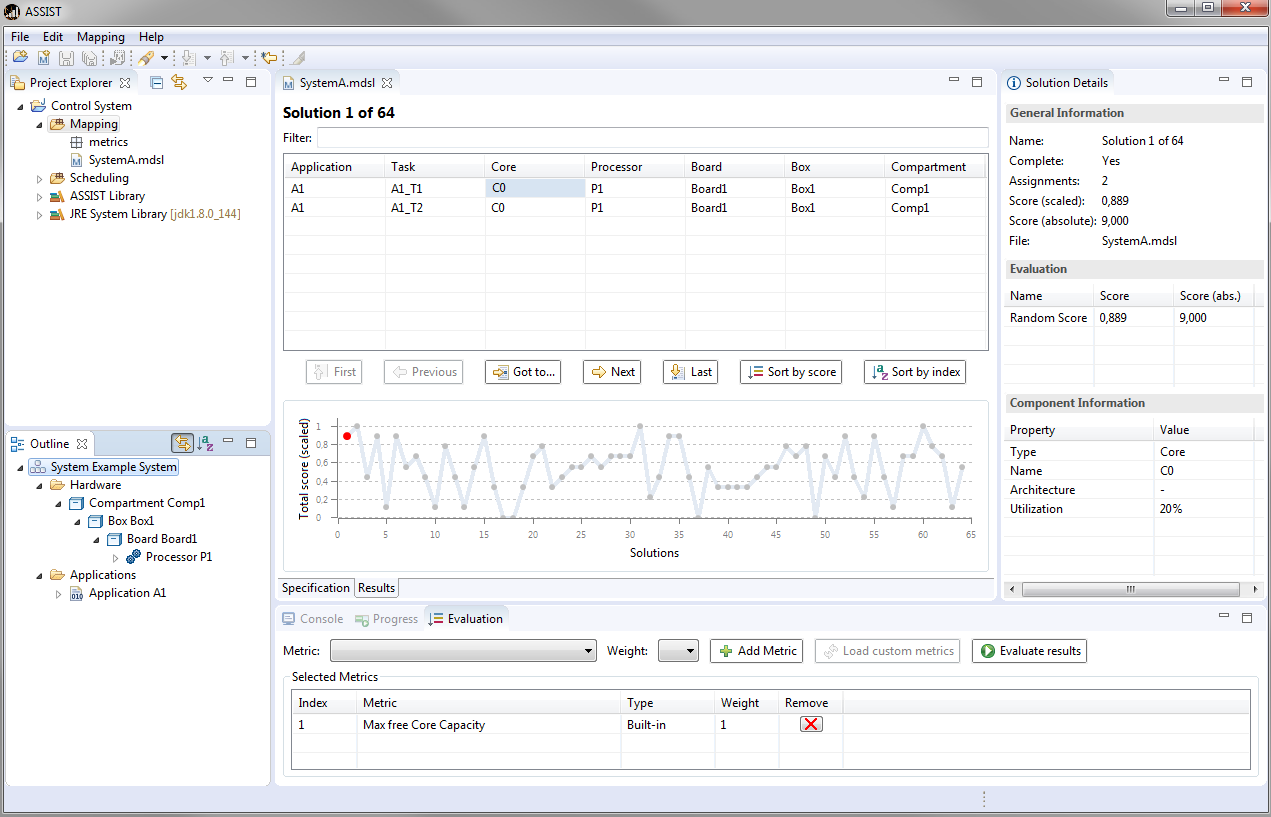
\includegraphics[width=\textwidth]{assist-screenshot}
\caption{Screenshot of the ASSIST User Interface}
\label{tool}
\end{figure}

ASSIST allows a systems engineer to automatically construct and optimize mappings based on textual specifications of the software components and hardware resources, \textit{dislocality}, \textit{dissimilarity} and \textit{colocality} requirements, and also optimization goals.
The textual specifications in ASSIST conform to a domain-specific language which allows to hide the intricacies of a formal specification.
%Using a domain-specific language is expedient to enable systems engineers without a formal education in computer science to precisely specify a deployment problem.

\section{Ensuring Fault Tolerance by Requiring Dislocality}

In order to achieve fault tolerance and reliability, it is essential to support ``significant differences'' in the choice of resources to which critical software components are deployed to.
For example, a simple redundancy requirement between two software components, may force the systems engineer to allocate these software components to different processing boards in different locations aboard an airplane.
Furthermore, systematic errors and undetected design flaws in hardware components may be addressed by choosing dissimilar hardware resources, processors or memory blocks from different vendors for example.

Due to the importance of choosing  ``different'' resources for fault tolerance and reliability in safety-critical systems, engineering tools for an automated construction of deployments need to be able to fully support these choices.
ASSIST supports the engineer by offering \emph{dislocality} and \emph{dissimilarity} requirements as part of the domain specific language.
They can be used to enforce ``differences'' for the choice of resources during the mapping process.
Finding an \emph{efficient} formulation to express the semantics of each requirement as a Constraint Satisfaction Problem is challenging, but also essential in order to provide an effective toolsuite for the engineering of safety-critical systems.

In order to illustrate the challenges and to present specific modeling improvements, the \emph{dislocality} requirement is used as an example in this paper.
Please note, that the concepts developed for \emph{dislocality} requirements can also be applied to \emph{dissimilarity} requirements.

The semantics of a dislocality requirement can be illustrated with the following deployment problem (see Figure~\ref{example}).
In this example system, there are three \emph{applications} consisting of one or more \emph{tasks}.
Each task has to be mapped to exactly one of the \emph{processors} in the system.
It is assumed, that the processor contains multiple cores, so that multiple tasks can be mapped to a single processor.
However, in order to ensure fault tolerance, a \emph{dislocality} requirement is added for all applications.
This means, that the applications must not share a processor, so that a faulty processor affects only one application.

\begin{figure}
\centering
\subcaptionbox{Simple Case}{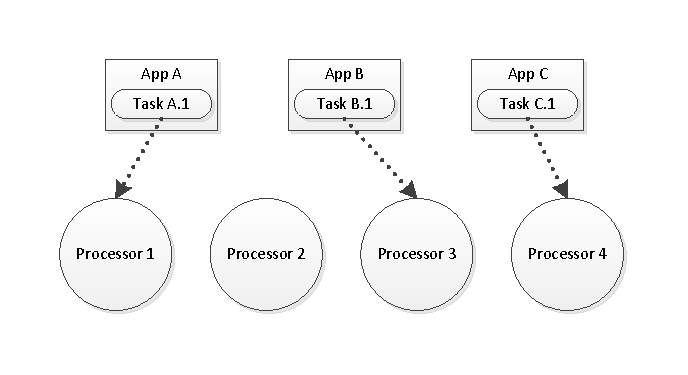
\includegraphics[width=0.47\textwidth]{application-mapping-simple}}%
\hfill
\subcaptionbox{Complex Case}{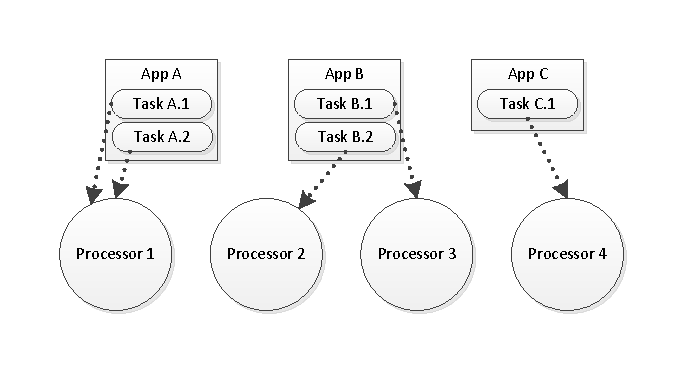
\includegraphics[width=0.47\textwidth]{application-mapping-complex}}%
\caption{An Example Deployment Problem - Mapping Tasks to Processors}
\label{example}
\end{figure}

Expressing the basic deployment problem with constraints is straight forward.
Each task~$i$ in the system is represented by an integer variable $X_i$.
The domain of each variable $X_i$ corresponds to the indices of the $n$ processors in the system ($X_i  \in \{0, 1, \dots, n-1\}$).
In order to add the constraints for the dislocality requirements, two cases have to be distinguished. 
In the simple case, in which all applications consist of only one task, a dislocality can be enforced with a single \texttt{allDifferent} constraint (see~\cite{GCCAT2014}) over all task variables $X_i$.
This case is depicted in Figure~\ref{example}~(a).
Fortunately, Choco 4 already contains an implementation for an \texttt{allDifferent} constraint based on the algorithm of Régin~\cite{Regin1994}, so that the simple case can be implemented.

In real-world systems, applications usually consist of more than one task.
Furthermore, tasks of the same application usually share the same processor.
This situation is more complex and depicted in Figure~\ref{example}~(b).
Unfortunately, in this case, the previous approach of applying a single \texttt{allDifferent} constraint over all task variables $X_i$ can no longer be used.
It would prevent solutions in which a processor is shared by multiple tasks of the same application.

The existing \texttt{allDifferent} constraint simply ensures, that values for a list of variables are different.
However, the complex case requires an advanced \texttt{allDifferent} constraint working with \emph{a list of a list of variables} and ensuring that the combined values for each list of variables are disjunct.
Unfortunately, such a constraint is neither part of the Global Constraint Catalog~\cite{GCCAT2014} nor available in Choco 4.

\section{Modeling Complex Dislocality Requirements}

This section introduces three alternative implementations for the semantics of an advanced \texttt{allDifferent} constraint.
Their performance and impact on resolution time will be analyzed and compared to each other in the next section.

Before continuing with the description of possible implementations, the semantics of an advanced \texttt{allDifferent} constraint should be described more precisely.
For this purpose, consider the example system in Figure~\ref{example}~(b).
It consists of the applications $A$, $B$ and $C$.
Each of these applications contains one or more tasks, i.e. $A = \{A_1, A_2\}$, $B = \{B_1, B_2\}$ and $C = \{C_1\}$.
An advanced \texttt{allDifferent} for all applications would be working with a list of a list of variables, for example:
$$\textrm{\texttt{allDifferent}}\left\{\{A_1, A_2\}, \{B_1, B_2\}, \{C_1\}\right\}$$
Assuming that $A^\star$ combines the values for each task in application $A$:
$$A^\star \in \mathcal{P}(\mathbb{N}) = \bigcup \left\{A_i : A_i \in A\right\} \qquad ( = A_1\cup A_2)$$
and $B^\star$ and $C^\star$ do the same for the applications $B$ and $C$, then the advanced \texttt{allDifferent} constraint would ensure, that the sets $A^\star$, $B^\star$ and $C^\star$ are pairwise disjunct.

\subsection*{Element-wise Approach}

One option to implement the advanced \texttt{allDifferent} constraint semantic is to apply the already existing \texttt{allDifferent} constraint for every subset $s$ with
$$s = \{a,b,c \, \vert \, a \in A,  b \in B, c \in C\}$$
For systems with a large amount of applications and more than one task within each application, the amount of constraints, that will be added to the constraint solver by this approach, may significantly prolong the resolution time.
However, this approach can be realized with the tools already available in Choco 4 and does not require any additional implementation of custom propagators and constraints\footnote{\url{https://github.com/RobertHilbrich/assist-public/blob/master/ch.hilbri.assist.mapping/src/ch/hilbri/assist/mapping/solver/constraints/DislocalityConstraint.xtend}}.

\subsection*{Instantiation-only Approach}

In order to address the drawbacks of the first approach, another option is to implement a custom constraint and propagator\footnote{\url{https://github.com/RobertHilbrich/assist-public/blob/master/ch.hilbri.assist.mapping/src/ch/hilbri/assist/mapping/solver/constraints/choco/PropAllDiffListsOfListsInst.java}} for Choco 4, that is able to operate on a list of a list of variables.
For the sake of simplicity, the propagator should only react on instantiation events for any of its variables.
If an instantiation is detected, then the value of the instantiated variable will be removed from the values of all variables in all of the \emph{other} lists.
This approach has the advantage, that only one constraint needs to be added to the constraint solver for each dislocality requirement.
However, this instantiation-only approach leads to a weak propagation as it only removes values, when one of the variables is instantiated.
%Therefore, this approach relies on the application of clever search strategies in order to be efficient.

\subsection*{Combined Union-Variables and Instantiation-Only Approach}

The third approach tries to build upon the instantiation-only approach and improve the strength of its propagation.
For this purpose, a new integer variable $X^\star$ will be added for each list of task variables $X = \{X_1, \dots, X_n\}$ that were provided to the advanced \texttt{allDifferent} constraint.
The new variable $X^\star$ will contain the union of the remaining values of all variables in $X$.
This can be achieved with a custom propagator\footnote{\url{https://github.com/RobertHilbrich/assist-public/blob/master/ch.hilbri.assist.mapping/src/ch/hilbri/assist/mapping/solver/constraints/choco/PropIntValuesUnion.java}} similar to the already existing \texttt{PropSetIntValuesUnion} propagator in Choco 4.
With these new ``union variables'' being available, adding a simple \texttt{allDifferent} constraint, which links all of the union variables, should improve the effectiveness of the propagation.
Please note, that these ``union variables'' must not be added to the list of variables for branching as part of the search strategy in Choco 4 as they will not always be resolved to only \emph{one} value if tasks of an application are deployed to different processors.
This approach will be combined with the instantiation-only approach from the previous section.
In comparison to the instantiation-only approach, the handling of union-variables requires the addition of a new variable and a propagator for each list of variables, so there is some overhead to be expected.

Based on the description of these three approaches to implement the semantics of an advanced \texttt{allDifferent} constraint, the next sections will describe experiments conducted by the authors and preliminary results to assess and compare the performance and efficiency of each approach.

\section{Experiments}

Benchmarking the performance and efficiency of these approaches requires several example to work on.
For this purpose, the authors developed a generator\footnote{\url{https://github.com/RobertHilbrich/assist-public/blob/master/ch.hilbri.assist.mapping.benchmarking/src/ch/hilbri/assist/mapping/benchmarking/generator/MappingExampleGenerator.xtend}} for synthetic mapping problems that resemble the typical characteristics of mapping problems encountered in safety-critical systems.
Twenty randomized examples\footnote{\url{https://github.com/RobertHilbrich/assist-public/tree/master/ch.hilbri.assist.mapping.tests/resources}} with at least one solution were generated for the experiments.
They exhibit the following properties\footnote{\url{https://github.com/RobertHilbrich/assist-public/blob/master/ch.hilbri.assist.mapping.tests/src/ch/hilbri/assist/mapping/tests/benchmarking/BenchmarkingTests.xtend}}.

In each example, there are \emph{two} compartments, each containing between \emph{four} and \emph{six} boxes.
Each box contains between \emph{four} and \emph{six} processing boards and every processing board is equipped with \emph{one} or \emph{two} processors each comprising of up to \emph{four} cores.
The examples contain between \emph{16} and \emph{24} applications and each of these applications have between \emph{two} and \emph{eight} tasks that need to be mapped to the cores on the processors.
All tasks of an application are required to be placed on the same processing board to allow for memory-based communication (colocality requirement).
Finally, every example features between \emph{24} and \emph{32} dislocality requirements and each of these requirements refers to at least \emph{four} and up to \emph{six} applications.

Every example was benchmarked on an Apple iMac 5k with 64GB of RAM by using ASSIST 2.3 and Choco 4.0.6.
The experiments were done with the \emph{Domain over Weighted Degree} as a variable selector strategy and \emph{Minimum Value First} as a value selector strategy.
The examples are publicly available in the ASSIST repository\footnote{\url{https://github.com/RobertHilbrich/assist-public/tree/master/ch.hilbri.assist.mapping.tests/resources}}.

\section{Results}

The amount of constraints and variables are depicted for each example and each approach in Figure~\ref{results-constraints-count} and Figure~\ref{results-variables-count}.
The results show, that the element-wise approach leads to a substantial increase in the amount of constraints in the solver in comparison to the other two approaches.
However, the increase of the variable count due to the addition of union-variables for the implementation of the third approach appears to be rather negligible.

\begin{figure}[h!tbp]
\centering
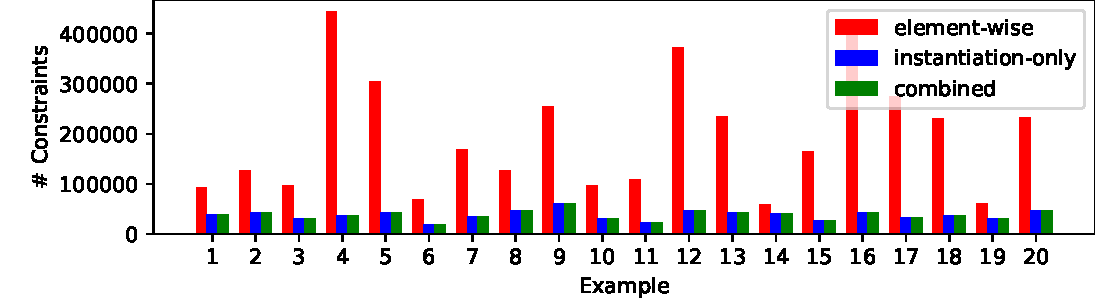
\includegraphics[width=\textwidth]{results-constraint-count}
\caption{Amount of constraints in the Choco solver in each example}
\label{results-constraints-count}
\vspace*{\floatsep}
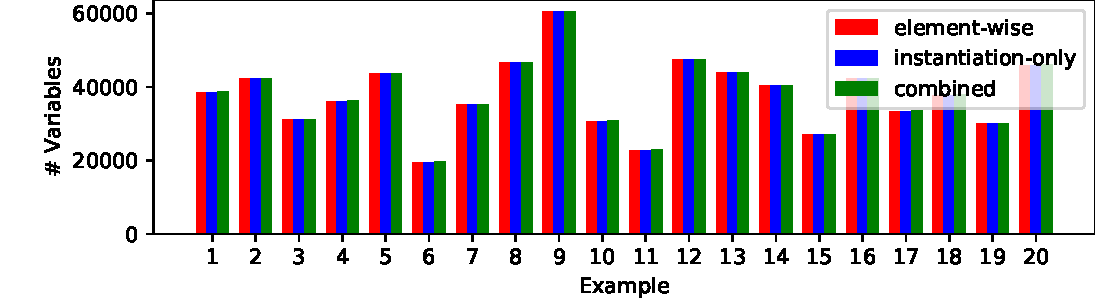
\includegraphics[width=\textwidth]{results-variables-count}
\caption{Amount of variables in the Choco solver in each example}
\label{results-variables-count}
\end{figure}

\begin{figure}[h!tbp]
\centering
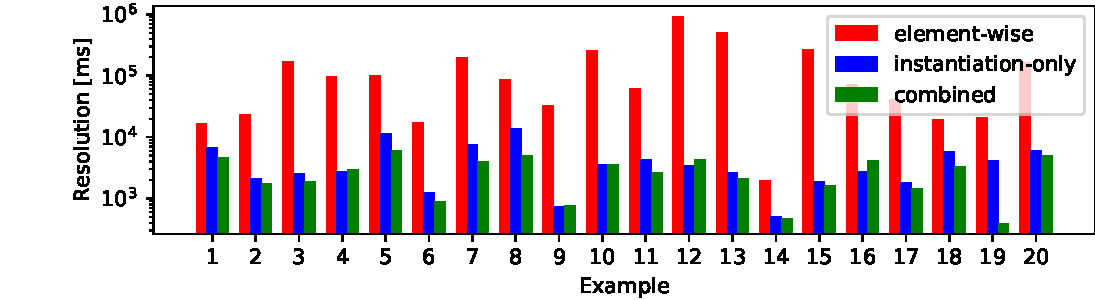
\includegraphics[width=\textwidth]{results-resolution}
\caption{Resolution time (in ms) to reach the first solution in each example}
\label{results-resolution}
\end{figure}

The total resolution time until the first solution has been reached is depicted in Figure~\ref{results-resolution}.
Please note the logarithmic scale on the y-axis.
The results demonstrate, that the resolution time can be significantly reduced in all examples by adopting the instantiation-only approach.
Further improvements to the instantiation-only approach can be achieved by applying the combined approach, but the additional gains are significantly smaller.
In some examples, the combined approach requires slightly more time for a resolution.
However, the time differences in these cases are so small, that they may also be induced by external effects, such as garbage collection in Java or scheduling interferences in the operating system.

\begin{figure}[h!tbp]
\centering
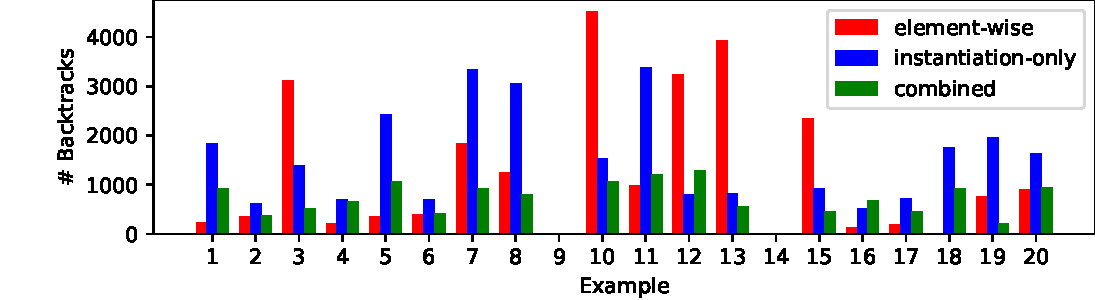
\includegraphics[width=\textwidth]{results-backtracks}
\caption{Amount of backtracking occurring in each example}
\label{results-backtracks}
\end{figure}

Backtracking occurs, when the search process in the constraint solver encounters a \emph{fail} event, i.e. a variable has an empty domain after value propagation or one of the constraints determines a contradiction.
Figure~\ref{results-backtracks} shows the amount of backtracking that occurred before finding the first solution in each example.
One would assume, that the element-wise approach exhibits the strongest propagation due to the large amount of additional \texttt{allDifferent} constraints, so that the amount of fails and backtracks might be smaller compared to the other approaches.
In fact, the results are not as clear-cut.
Some examples show, that the propagation of the element-wise approach is significantly stronger compared to the other approaches.
However, there are also other examples in which the situation is reversed.

\section{Summary and Conclusions}

Ensuring significant differences in the choice of resources to which software components in safety-critical systems are deployed to, is essential for satisfying safety requirements and facilitating fault tolerance.
ASSIST is a toolsuite for system engineers, which aims to automate the deployment of software components to hardware resources by transforming this mapping problem into an equivalent Constraint Satisfaction Problem.
In ASSIST, there are several means to require ``differences'' in the choice of resources.
\emph{Dislocality} requirements are one of those means and they are used as an example in this paper to illustrate the challenge of finding an efficient constraint model.

Three different approaches to implement the intended semantics of dislocality requirements are presented.
They specifically address complex use-cases in which applications consist of multiple tasks.
While one of these approaches can be realized without any customized constraints or propagators, the other two approaches rely on custom implementations of constraints and propagators as well as additional variables in the third approach.

Experiments conducted with twenty synthesized mapping examples for ASSIST show, that the implementation of custom constraints and propagators is well worth the effort.
They lead to a substantial reduction in the resolution time with only minimal overhead due to the additional constraints and variables.
The results also indicate, that the element-wise approach, which requires the highest amount of additional constraints, does not always lead to the lowest rate of backtracks in the examples.

\section*{Acknowledgment}

The authors acknowledge the financial support for this work by the Federal Ministry of Education and Research of Germany (BMBF) in the project ``ARAMiS II'' (DLR, grant identifier 01IS16025D).


\printbibliography[heading=bibintoc]

\end{document}

%%% Local Variables: 
%%% mode: latex
%%% TeX-master: "paper"
%%% ispell-check-comments: exclusive
%%% ispell-local-dictionary: "english"
%%% End:
